%%%%%%%%%%%%%%%%%%%%%%%%%%%%%%%%%%%%%%
% LaTeX poster template
% Created by Nathaniel Johnston
% August 2009
% http://www.nathanieljohnston.com/2009/08/latex-poster-template/
%%%%%%%%%%%%%%%%%%%%%%%%%%%%%%%%%%%%%%

\documentclass[final]{beamer}
\usepackage[scale=1.24]{beamerposter}
\usepackage{graphicx}			% allows us to import images
\usepackage{anyfontsize}

%-----------------------------------------------------------
% Define the column width and poster size
% To set effective sepwid, onecolwid and twocolwid values, first choose how many columns you want and how much separation you want between columns
% The separation I chose is 0.024 and I want 4 columns
% Then set onecolwid to be (1-(4+1)*0.024)/4 = 0.22
% Set twocolwid to be 2*onecolwid + sepwid = 0.464
%-----------------------------------------------------------

\newlength{\sepwid}
\newlength{\onecolwid}
\newlength{\twocolwid}
\newlength{\threecolwid}
\setlength{\paperwidth}{48in}
\setlength{\paperheight}{44.5in}
\setlength{\sepwid}{0.024\paperwidth}
\setlength{\onecolwid}{0.275\paperwidth}
\setlength{\twocolwid}{0.575\paperwidth}
\setlength{\threecolwid}{0.6\paperwidth}
\setlength{\topmargin}{-0.5in}
\usepackage[]{moresize}
\usetheme{confposter}
\usepackage{exscale}

%-----------------------------------------------------------
% The next part fixes a problem with figure numbering. Thanks Nishan!
% When including a figure in your poster, be sure that the commands are typed in the following order:
% \begin{figure}
% \includegraphics[...]{...}
% \caption{...}
% \end{figure}
% That is, put the \caption after the \includegraphics
%-----------------------------------------------------------

\usecaptiontemplate{
\small
\structure{\insertcaptionname~\insertcaptionnumber:}
\insertcaption}

%-----------------------------------------------------------
% Define colours (see beamerthemeconfposter.sty to change these colour definitions)
%-----------------------------------------------------------

\setbeamercolor{block title}{fg=ngreen,bg=white}
\setbeamercolor{block body}{fg=black,bg=white}
\setbeamercolor{block alerted title}{fg=white,bg=dblue!70}
\setbeamercolor{block alerted body}{fg=black,bg=dblue!10}

%-----------------------------------------------------------
% Name and authors of poster/paper/research
%-----------------------------------------------------------

\title{{\fontsize{111}{111}\selectfont Near-inertial waves} {extract energy}
{\fontsize{75}{75}\selectfont from}\\ \hskip2.5cm {\fontsize{75}{75}\selectfont barotropic}
        {\fontsize{111}{111}\selectfont quasi-geostrophic flow}$^\dagger$ }
\author{\textbf{Cesar B. Rocha} and Gregory L. Wagner and William R. Young}
\institute{\hskip1.25cm crocha\textbf{@ucsd}.edu\hskip2.5cm
           \hskip3.75cm glwagner\textbf{@mit}.edu \hskip2.5cm
           \hskip2.5cm wryoung\textbf{@ucsd}.edu \hskip2.5cm
          }

% adds art to title box
           \setbeamertemplate{headline}{
            \leavevmode
            \begin{columns}
              \begin{column}{.6\linewidth}
               \vskip1cm
               \hskip2.cm
               \usebeamercolor{title in headline}{\color{jblue}\Huge{\textbf{\inserttitle}}\\[0.5ex]}
               \hskip2.5cm
               \usebeamercolor{author in headline}{\color{fg}\Large{\insertauthor}\\[1ex]}
               \hskip2.cm
               \usebeamercolor{institute in headline}{\color{fg}\large{\insertinstitute}\\[1ex]}
               \vskip1cm
              \end{column}
              \begin{column}{.4\linewidth}
                \hspace{17.em}
                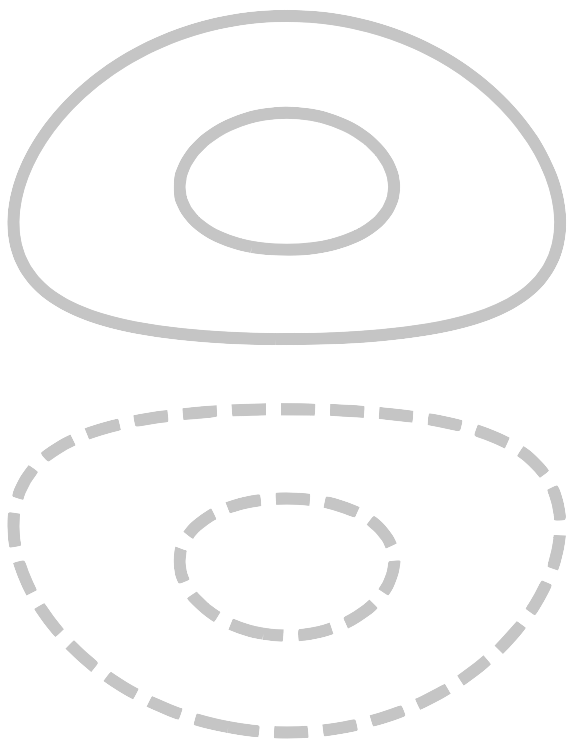
\includegraphics[width=0.2\linewidth]{figs/dipole2art_1.png}\hspace{.5em}
                %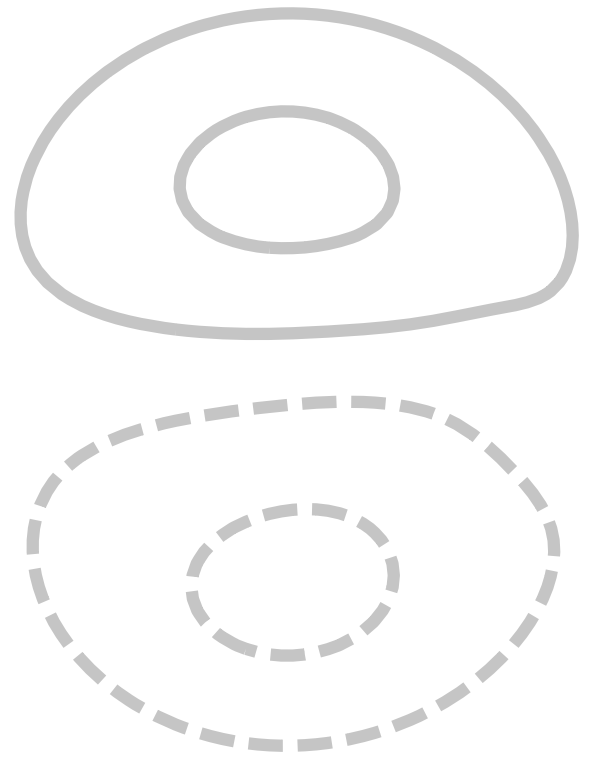
\includegraphics[width=0.2\linewidth]{figs/dipole2art_2.png}\hspace{1.5em}
               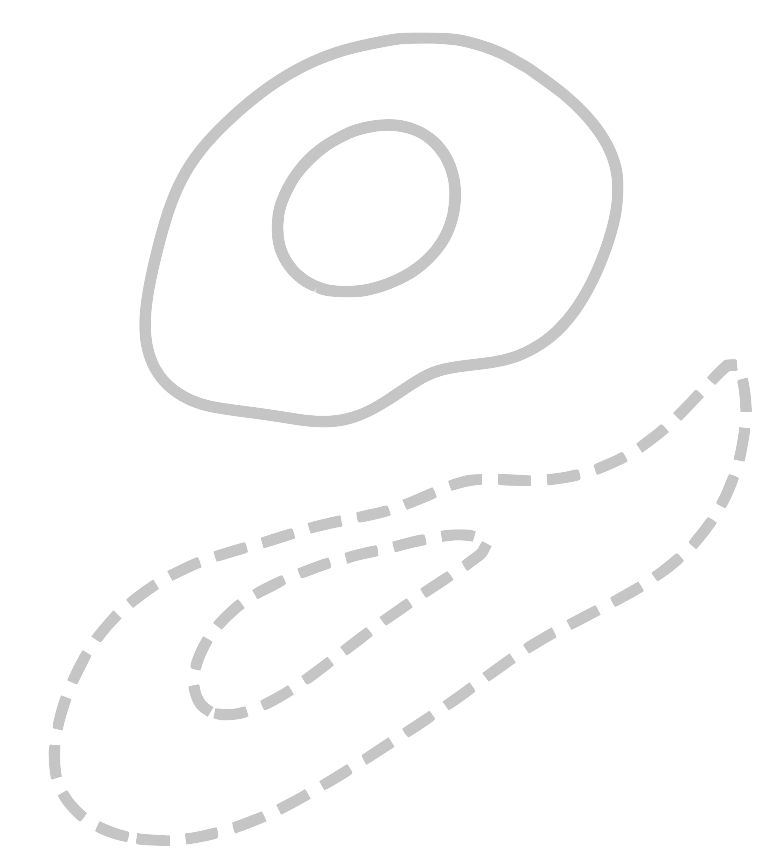
\includegraphics[width=0.25\linewidth]{figs/dipole2art_3.png}\hspace{-6.em}
               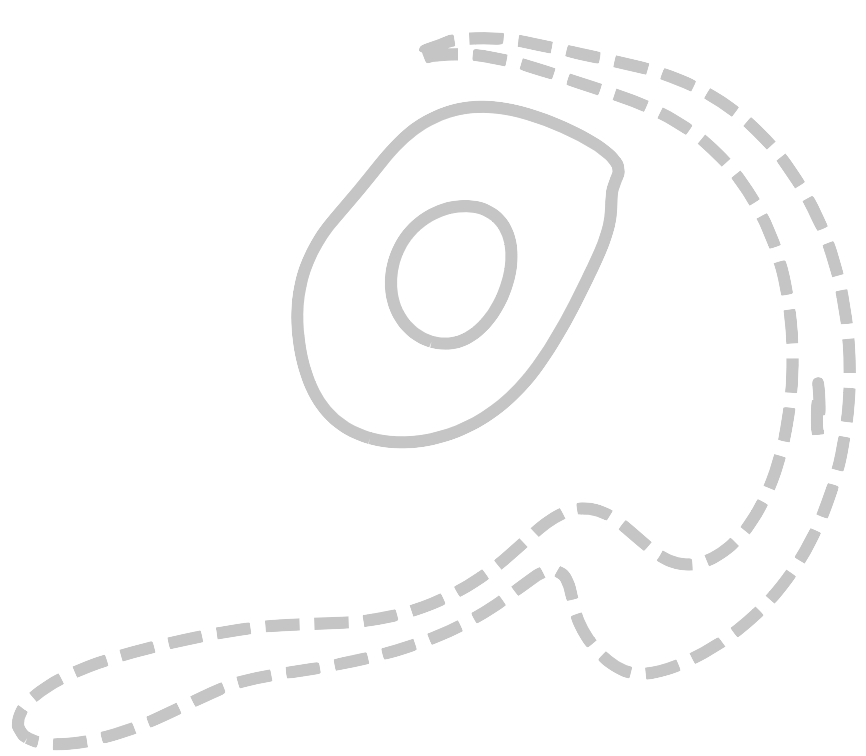
\includegraphics[width=0.315\linewidth]{figs/dipole2art_4.png}
              \end{column}
              \vspace{1cm}
             \end{columns}
            \vspace{.2cm}
            \hspace{0.5in}\begin{beamercolorbox}[wd=46in,colsep=0.15cm]{cboxb}\end{beamercolorbox}

            \vspace{0.1in}
           }


%-----------------------------------------------------------
% Start the poster itself
%-----------------------------------------------------------

\begin{document}


\newcommand{\com}{\, ,}
\newcommand{\per}{\, .}

%% Averages
% Use \bar to over line solo symbols

\newcommand{\av}[1]{\bar{#1}}
\newcommand{\avbg}[1]{\overline{#1}}
\newcommand{\avbgg}[1]{\overline{#1}}

% A nice definition
\newcommand{\defn}{\ensuremath{\stackrel{\mathrm{def}}{=}}}

% space in equations
\newcommand{\qqand}{\qquad \text{and} \qquad}
\newcommand{\qand}{\quad \text{and} \quad}

% equations
\def\beq{\begin{equation}}
\def\eeq{\end{equation}}

\def\bea{\begin{align}}
\def\ena{\end{align}}


% calculus
\newcommand{\ord}{\mathcal{O}}
%\newcommand{\p}{\partial}
\newcommand{\ii}{{\rm i}}
\newcommand{\dd}{{\rm d}}
\newcommand{\id}{{\, \rm d}}
\newcommand{\ee}{{\rm e}}
\newcommand{\DD}{{\rm D}}
\newcommand{\wavy}{\text{wavy}}
\newcommand{\qg}{\text{qg}}
\newcommand{\dt}{\Delta t}
\newcommand{\dx}{\Delta x}
\newcommand{\be}{\beta}

\newcommand{\al}{\alpha}
\newcommand{\bx}{\boldsymbol{x}}
\newcommand{\by}{\boldsymbol{y}}
\newcommand{\bu}{\boldsymbol{u}}
\newcommand{\bv}{\boldsymbol{v}}


\newcommand{\half}{\tfrac{1}{2}}
\newcommand{\halfi}{\tfrac{\ii}{2}}
\newcommand{\quarter}{\tfrac{1}{4}}
\newcommand{\quarteri}{\tfrac{\ii}{4}}
\newcommand{\halfrho}{\tfrac{1}{2}}
\newcommand{\rz}{{}}
\newcommand{\bn}{\boldsymbol{\hat n}}
\newcommand{\br}{\boldsymbol{r}}
\newcommand{\bR}{\boldsymbol{R}}
\newcommand{\bA}{\ensuremath {\boldsymbol {A}}}
\newcommand{\bB}{\ensuremath {\boldsymbol {B}}}
\newcommand{\bU}{\ensuremath {\boldsymbol {U}}}
\newcommand{\bE}{\ensuremath {\boldsymbol {E}}}
\newcommand{\bN}{\ensuremath {\boldsymbol {\mathrm{N}}}}
\newcommand{\bJ}{\ensuremath {\boldsymbol {J}}}
\newcommand{\bXX}{\ensuremath {\boldsymbol {\mathcal{X}}}}
\newcommand{\bFF}{\ensuremath {\boldsymbol {F}}}
\newcommand{\bF}{\ensuremath {\boldsymbol {F}^{\sharp}}}
\newcommand{\bG}{\ensuremath {\boldsymbol G}}
\newcommand{\bSigma}{\ensuremath {\boldsymbol {\Sigma}}}
\newcommand{\bvarphi}{\ensuremath {\boldsymbol {\varphi}}}
\newcommand{\bxi}{\ensuremath {\boldsymbol {\xi}}}
\newcommand{\avbxi}{\overline{\ensuremath {\boldsymbol {\xi}}}}

% math cal

\newcommand{\J}{\mathcal{J}}
\newcommand{\K}{\mathcal{K}}
\newcommand{\cG}{\mathcal{G}}
\newcommand{\cF}{\mathcal{F}}
\newcommand{\cN}{\mathcal{N}}
\newcommand{\cL}{\mathcal{L}}
\newcommand{\cS}{\mathcal{S}}
\newcommand{\cE}{\mathcal{E}}


% san serif for matrices and differential operators
%\newcommand{\helmn}{\mathsf{H}_n}
\newcommand{\helmm}{\triangle_m}
\newcommand{\helmn}{\triangle_n}
\newcommand{\helms}{\triangle_s}
\newcommand{\helm}{\triangle}
\newcommand{\sA}{\mathsf{A}}
\newcommand{\sB}{\mathsf{B}}
\newcommand{\sG}{\mathsf{G}}
\newcommand{\sI}{\mathsf{I}}
%\newcommand{\sJ}{\mathsf{J}}
\newcommand{\sJ}{J}
\newcommand{\gsJ}{\breve{\mathsf{J}}}
\newcommand{\sU}{\mathsf{U}}
\newcommand{\sP}{\mathsf{P}}
\newcommand{\sQ}{\mathsf{Q}}
\newcommand{\sR}{\mathsf{R}}
\newcommand{\sL}{\mathsf{L}}
\newcommand{\Lu}{\mathsf{L}(\what{u}_k)}
\newcommand{\Nu}{\mathsf{N}(\what{u}_k)}
\renewcommand{\L}{\mathsf{L}}
\newcommand{\N}{\mathsf{N}}
\newcommand{\sH}{\mathsf{H}}
\renewcommand{\sI}{\mathsf{I}}
\renewcommand{\L}{\mathsf{L}}
\newcommand{\sM}{\mathsf{M}}
\newcommand{\sT}{\mathsf{T}}
\newcommand{\sGamma}{\mathsf{\Gamma}}
\newcommand{\sOmega}{\mathsf{\Omega}}
\newcommand{\sSigma}{\mathsf{\Omega}}
\newcommand{\sbeta}{\mathsf{\beta}}
\newcommand{\sPi}{\mathsf{\Pi}}
\newcommand{\sC}{\mathsf{C}}
\newcommand{\sQy}{\mathsf{Q}}
\renewcommand{\sb}{\mathsf{b}}

% u
\newcommand{\uhat}{\what{u}_k}

% angle brackets

\def\la{\langle}
\def\ra{\rangle}
\def\laa{\left \langle}
\def\raa{\right \rangle}


%grads and div's
%\newcommand{\bcdot}{\hspace{-0.1em} \boldsymbol{\cdot} \hspace{-0.12em}}
%\newcommand{\bnabla}{\boldsymbol{\nabla}}
\newcommand{\bnablaH}{\bnabla_{\! \mathrm{h}}}
\newcommand{\grad}{\bnabla}
\newcommand{\gradH}{\bnablaH}
\newcommand{\curl}{\bnabla \!\times\!}
\newcommand{\diver}{\bnabla \! \bcdot \! }
\newcommand{\cross}{\times}
%\newcommand{\lap}{\nabla^2}
\newcommand{\lap}{\triangle}

%varthetas and thetas
\newcommand{\vth}{\vartheta}
\newcommand{\psii}{\psi^{\mathrm{i}}}
\newcommand{\thb}{\theta^{\mathrm{-}}}
\newcommand{\vthb}{\vartheta^{\mathrm{-}}}
\newcommand{\vthbhat}{{\hat{\vartheta}}^{\mathrm{-}}}
\newcommand{\vThb}{\varTheta^{\mathrm{-}}}
\newcommand{\psib}{\psi^{\mathrm{-}}}
\newcommand{\tht}{\theta^{\mathrm{+}}}
\newcommand{\vtht}{\vartheta^{\mathrm{+}}}
\newcommand{\vththat}{{\hat{\vartheta}}^{\mathrm{+}}}
\newcommand{\vthtbhat}{{\hat{\vartheta}}^{\pm}}
\newcommand{\vTht}{\varTheta^{\mathrm{+}}}
\newcommand{\vthtb}{\vartheta^{\pm}}
\newcommand{\vThtb}{\varTheta^{\pm}}

% nondimensional numbers
\renewcommand{\Re}{\mathrm{Re}}
\newcommand{\Ro}{\mathrm{Ro}}
\newcommand{\Bu}{\mathrm{Bu}}
\newcommand{\Ri}{\mathrm{Ri}}

%psi's
%Galerking coefficient for psi:
\newcommand{\gpsi}{\breve \psi}
\newcommand{\gpsic}{{\breve \psi}^\star}
\newcommand{\gtau}{\breve \tau}
\newcommand{\gtauc}{{\breve \tau}^\star}
\newcommand{\gphi}{\breve \phi}
\newcommand{\gq}{\breve q}
\newcommand{\gU}{\breve U}
\newcommand{\gQ}{\breve Q}
\newcommand{\gsigma}{\breve \sigma}


\newcommand{\psit}{\psi^{\mathrm{+}}}
\newcommand{\psithat}{{\hat{\psi}}^{\mathrm{+}}}
\newcommand{\psibhat}{{\hat{\psi}}^{\mathrm{-}}}
\newcommand{\psitb}{\psi^{\pm}}
\newcommand{\psitbhat}{{\hat{\psi}}^\pm}
\newcommand{\St}{S^{\mathrm{+}}}
\newcommand{\Sb}{S^{\mathrm{-}}}
\newcommand{\phb}{\phi^{\mathrm{-}}}
\newcommand{\pht}{\phi^{\mathrm{+}}}
\newcommand{\tautb}{\tau^{\pm}}
\newcommand{\sigmatb}{\sigma^{\pm}}


\newcommand{\bur}{\left(\tfrac{f_0}{N}\right)^2}
\newcommand{\ibur}{\left(\tfrac{N}{f_0}\right)^2}
\newcommand{\Nm}{N_{\mathrm{mix}}}
\newcommand{\xim}{\xi_{\mathrm{mix}}}
\newcommand{\hs}{h_*}
\renewcommand{\sp}{\mathsf{p}}
\newcommand{\se}{\mathsf{e}}
\newcommand{\sptb}{\mathsf{p}^\pm}


%nmax is a problem:
%\newcommand{\nmax}{n_{\mathrm{max}}}
\newcommand{\nmax}{\mathrm{N}}
\newcommand{\mmax}{\mathrm{M}}

\newcommand{\WKB}{\mathrm{WKB}}
\newcommand{\Lam}{\Lambda}
\newcommand{\tha}{\theta}
\newcommand{\kap}{\kappa}
\newcommand{\bphi}{\boldsymbol{\phi}}
\newcommand{\third}{\tfrac{1}{3}}
\newcommand{\cs}{c^\star}
\newcommand{\dstar}{{\star\star}}
\newcommand{\nt}{n^{\mathrm{trnc}}}
\newcommand{\sDp}{\mathsf{D}^1_{\nmax}}
\newcommand{\sDpp}{\mathsf{D}^2_{\nmax}}
\newcommand{\sD}{\mathsf{D}}
\newcommand{\sDN}{\mathsf{D_\nmax}}
\newcommand{\sK}{\mathsf{K_2}}
\newcommand{\stheta}{\mathsf{\theta}}
\newcommand{\sphi}{\mathsf{\phi}}
\newcommand{\sq}{\mathsf{q}}
\newcommand{\cosech}{\text{csch}\,}
\newcommand{\sinc}{\text{sinc}\,}

%%%%%%%%% %%%%

%%%%%%%%% %%%%
\newcommand{\zt}{z^+}
\newcommand{\zb}{z^-}
\newcommand{\qA}{q^A_{\nmax}}
\newcommand{\psiB}{\psi^B_{\nmax}}
\newcommand{\phiB}{\phi^B_{\nmax}}
\newcommand{\eye}{\boldsymbol{\hat{i}}}
\newcommand{\jay}{\boldsymbol{\hat{j}}}
\newcommand{\kay}{\boldsymbol{\hat{k}}}
\newcommand{\psiG}{\psi^{\mathrm{G}}}
\newcommand{\qG}{q^{\mathrm{G}}}
\newcommand{\uG}{u^{\mathrm{G}}}
\newcommand{\UG}{U^{\mathrm{G}}}
\newcommand{\UGN}{U^{\mathrm{G}}_{\nmax}}
\newcommand{\QGN}{Q^{\mathrm{G}}_{\nmax}}
\newcommand{\sumoddn}{\sum_{n = 1, n~ \text{odd}}^{\nmax}}

% bretherton
\newcommand{\qBr}{q_{\mathrm{Br}}}
\newcommand{\psiBr}{\psi_{\mathrm{Br}}}

\newcommand{\ep}{\epsilon}
\newcommand{\vep}{\varepsilon}


%\renewcommand{\sZ}{\mathsf{Z}}
%\renewcommand{\sE}{\mathsf{E}}
\newcommand{\iBu}{\left(\tfrac{f_0}{N}\right)^2}
\newcommand{\F}{\mathcal{F}}
\newcommand{\D}{\mathcal{D}}
\newcommand{\phis}{\phi^\star}
\newcommand{\Ff}{\mathbf{F}}
\newcommand{\Sf}{\mathbf{S}}
\newcommand{\ut}{\mathbf{u}^\#}
\newcommand{\cg}{\mathbf{c}_g}
\newcommand{\Uf}{\mathbf{U}}
\renewcommand{\Im}{\mathrm{Im}}
\renewcommand{\div}{\nabla\cdot}
\renewcommand{\P}{\mathcal{P}}
\newcommand{\dU}{\delta U}
\newcommand{\W}{\mathcal{W}}
\newcommand{\cK}{\mathcal{K}}
\newcommand{\cP}{\mathcal{P}}
\renewcommand{\L}{\mathsf{L}}
\renewcommand{\N}{\mathsf{N}}
\newcommand{\psiq}{\psi^q}
\newcommand{\psiw}{\psi^w}
\newcommand{\p}{\partial}
\renewcommand{\defn}{\equiv}

\begin{frame}[t]

  \vspace{-1cm}

  \begin{columns}[t]												% the [t] option aligns the column's content at the top
    \begin{column}{\sepwid}\end{column}			% empty spacer column

    %\hspace{-2cm}
    \begin{column}{0.425\paperwidth}

      {
      \begin{alertblock}{Goal: to illuminate the physics of stimulated imbalance}
      Our goal is to understand the physics of stimulated imbalance---the transfer of energy
      from quasi-geostrophic flow to \textit{existing} near-inertial waves---associated
      with vertical vorticity and lateral strain.
      \end{alertblock}
      }

      \vskip1ex

      \begin{block}{The Xie \& Vanneste (2015) minimal model}

        With barotropic quasi-geostrophic flow, $\psi=\psi(x,y,t)$,
        uniform background buoyancy frequency, $N_0$,
        single-mode near-inertial vertical structure, $
        \ee^{\ii m z}$, and $\beta = 0$, the Xie \& Vanneste$^1$ coupled model (cf. Wagner \& Young, 2016$^2$)
         reduces to
        \beq
        \label{macroturb}
        q_t + \sJ(\psi,q) = D_q\qquad\text{with}\qquad
        q = \lap \psi +
                         \tfrac{1}{f_0}\Big[ \tfrac{1}{4} \lap |\phi|^2 + \tfrac{\ii}{2}
                         \sJ(\phi^\star,\phi)\Big]\com
        \eeq
        where $q$ is the \textit{wave-averaged} quasi-geostrophic potential vorticity
        (cf. Wagner \& Young, 2015$^3$), and
        \beq
        \label{waves}
        \phi_t + \underbrace{\sJ(\psi,\phi)}_{\text{Advection}} + \underbrace{\tfrac{\ii}{2}
        \phi\lap \psi}_{\text{Refraction}} - \underbrace{\tfrac{\ii}{2} f_0 \lambda^2
         \lap \phi}_{\text{Dispersion}}
         = D_\phi\qquad\text{with}\qquad u_w+\ii v_w  =
         \ee^{\ii (m z - f_0 t)} \phi(x,y,t)\com
        \eeq

        Above, $\psi$ is the streamfunction, $\lap \defn \p_x^2 + \p_y^2$,
        $\sJ(f,g)=f_x g_y - f_y g_x$, $^\star$ denotes complex conjugation,
        $\lambda = \tfrac{N_0}{f_0\, m}$, and the D-terms represent dissipation.
        The wave kinetic energy density satisfies

        \beq
        \label{action_density}
        \p_t \half |\phi|^2 + \sJ(\psi,\half|\phi|^2) + \diver \big(\underbrace{f_0
        \lambda^2\grad\Theta\,\,\,\half |\phi|^2}_{\defn\Ff_w}\big) = \text{dissipation}
        \com
        \eeq

        where $\Ff_w$ is the wave flux of kinetic energy density and
        $\phi = |\phi|\ee^{\ii\Theta}$.

        \end{block}
      \vskip2ex

      {
      \setbeamercolor{block alerted title}{fg=black,bg=ngreen} % Change the alert block title colors
      \setbeamercolor{block alerted body}{fg=black,bg=white} % Change the alert block body colors
      \begin{alertblock}{The physics of stimulated imbalance}

                From \eqref{waves}, we derive an equation for the wave potential energy,
                $P_w \defn \tfrac{1}{4}\lambda^2 \la|\nabla\phi|^2\ra$:

                \begin{align}
                \label{Pw}
                 \dot P_w =
                & \underbrace{\tfrac{1}{f_0}\Big\la\half\lap\psi\diver\Ff_w
                \Big\ra}_{\defn\Gamma_{r}} +
                \underbrace{\tfrac{\lambda^2}{2}\, \Big\la\half\psi\left[\sJ(\phi,\lap\phis)
                + \sJ(\phis,\lap\phi)\right]\Big\ra}_{\defn\Gamma_a}
                \, +\,\, \text{dissipation} \com
                \end{align}
                where $\la\,\,\ra$ represents horizontal average, and $\Gamma_r+\Gamma_a$ is the wave-potential energy generation, which occurs
                at the expenses of geostrophic kinetic energy, $K_e \defn \half \la|\nabla\psi|^2\ra$,
                i.e., $\dot K_e = -(\Gamma_r+\Gamma_a) + \text{dissipative terms}.$

                \begin{columns}
                  \begin{column}{.425\textwidth}
                  \begin{figure}
                    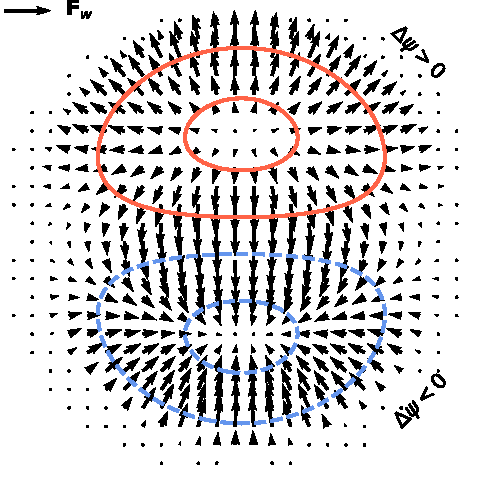
\includegraphics[width=0.75\textwidth]{figs/Gamma_r.pdf}
                    \caption{Snapshot of a solution of (1)-(2) with initially dipolar
                              geostrophic flow and uniform wave velocity
                              (cf. poster's art). Contours represents relative vorticity, $\lap\psi$,
                              and vectors depict the wave flux, $\Ff_w$.
                              \textbf{Refraction attracts (expels)
                              wave kinetic energy to anti-cyclones (from cyclones),
                              thereby generating wave potential energy at the expenses
                              of geostrophic kinetic energy ($\Gamma_r>0$)}.
                              }
                  \end{figure}
                \end{column}

                \begin{column}{0.535\textwidth}
                  \vskip1.75cm
                  \begin{figure}
                    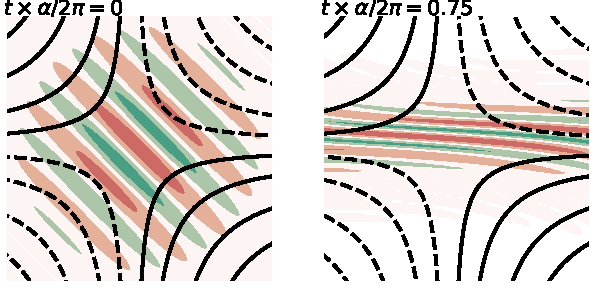
\includegraphics[width=0.95\textwidth]{figs/Gamma_a.pdf}
                    \caption{The distortion of a wave packet by an elongation flow,
                    $\psi = -\alpha xy$.
                    Black contours depict the
                    streamfunction, $\psi$, and colors represent the zonal wave velocity,
                    $u_w$.
                              \textbf{Geostrophic straining enhances gradients of $\phi$,
                              thereby generating wave potential energy at the expenses
                              of geostrophic kinetic energy ($\Gamma_a>0$)}. The
                              process is analogous to the generation tracer-gradient
                              variance by lateral straining. In the WBK limit, this
                              distortion resembles the `wave capture' mechanism of
                              B{\"u}hler \& McIntyre (2005).$^4$}
                  \end{figure}
                \end{column}

                \end{columns}
      \end{alertblock}
      }
      \vskip0.5cm
      ~~~~~~~$\dagger$ A manuscrupit in preparation. (Preprint soon on our websites.)\\
      ~~~~~~~~~Supported by NASA (NNX16AO5OH) and NSF (OCE1357047).
    \end{column}


    %
    % Second big column
    %
    \hspace{1.cm}

    \begin{column}{0.55\textwidth}

              \begin{block}{Macroturbulence solutions on a periodic domain}

                ~~~~~\textbf{Initial conditions}: uniform wave speed (inertial oscillation), $U_w$, and
                decaying barotropic turbulence flow emergent\\
                ~~~~~from random field with energy-containing wavenumber $k_e$,
                \beq
                \label{psi_init}
                |\hat{\psi}| = C \times \big\{|k|\,[1 + (|k|/k_e)^4]\big\}^{-1/2}
                \qquad\text{with}\qquad\sum_{k,l}
                 {|k|^2 |\hat{\psi}|^2} = \tfrac{1}{2}U_e^2\per
                \eeq
              ~~~~~\textbf{Two parameters}:
                \beq
                \label{alpha}
                \text{Amplitude:\,\,}\alpha \defn {\frac{U_e k_e}{f_0}} \times
                {\left(\frac{U_w}{U_e}\right)^2}\,;\qquad\text{Dispersivity:\,\,}
                \hslash \defn f_0 \lambda^2 \times \frac{k_e}{U_e}\per
                \eeq

              \end{block}

                      \begin{columns}
                        \begin{column}{.475\textwidth}

                        \begin{figure}
                          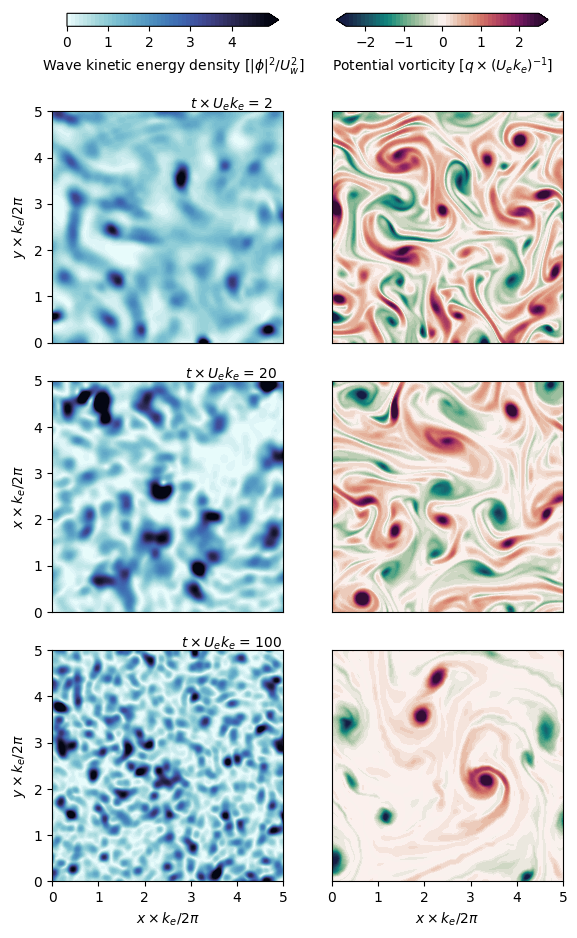
\includegraphics[width=0.8\textwidth]{figs/snapshots_turbulence.png}
                          \caption{Snapshots of solution with $\hslash \approx 1$
                                  and $\alpha \approx 1$. Left panels: wave kinetic energy density.
                                  Right panels: potential vorticity. These plots only show the bottom-left
                                 $(1/2)^2$ of the simulation domain.}
                        \end{figure}

                        \begin{figure}
                          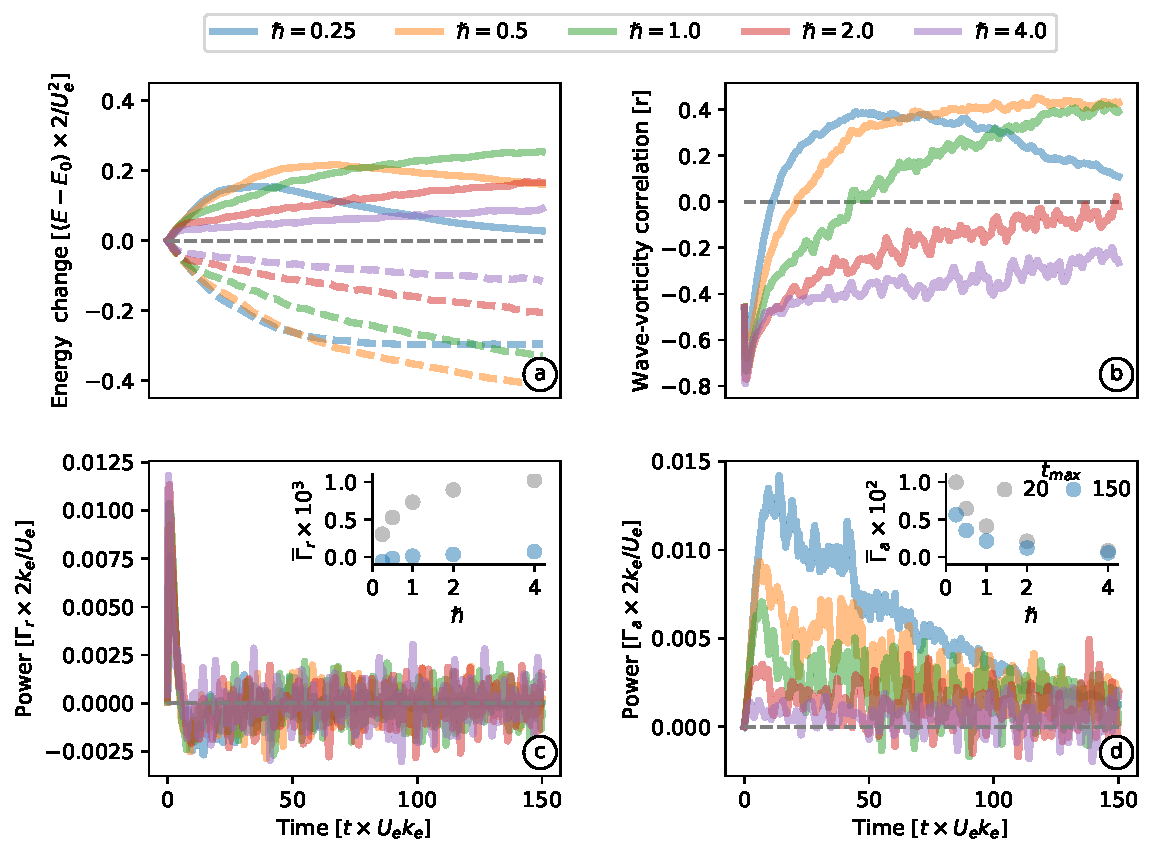
\includegraphics[width=0.95\textwidth]{figs/hslash_dependence_turbulence.pdf}
                          \caption{(a) Energy change about initial condition.
                                  (b)  Correlation between
                                  incoherent wave
                                  kinetic energy and relative vorticity.$^4$ Wave potential
                                  energy generation
                                  due to geostrophic refraction, $\Gamma_a$ (c) and advection, $\Gamma_r$ (d).}
                        \end{figure}

                      \end{column}

                      \hspace{0.cm}

                      \begin{column}{0.475\textwidth}

                        \begin{figure}
                          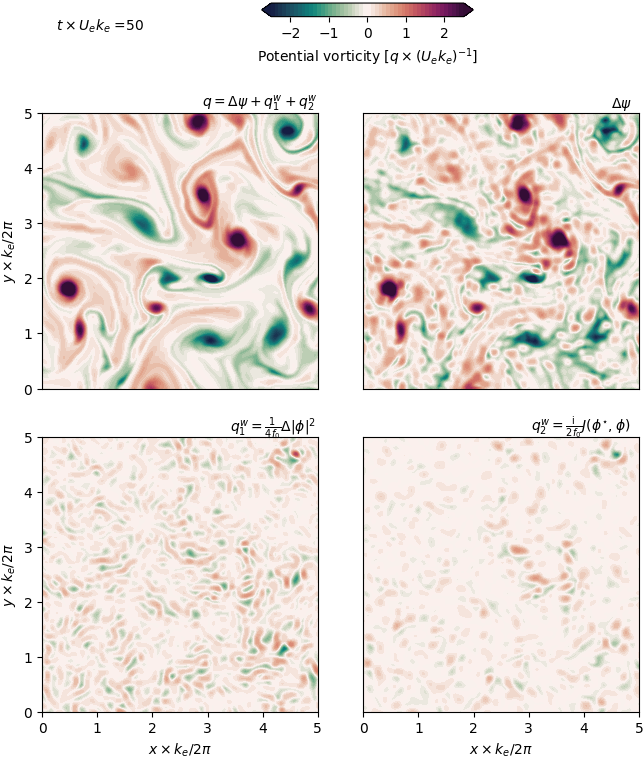
\includegraphics[width=0.85\textwidth]{figs/pv-terms_turbulence.png}
                          \caption{Snapshot of quasi-geostrophic potential vorticity
                                   of the decaying turbulence solution with $\hslash \approx 1$
                                   and $\alpha \approx 1$, at $t\times U_e k_e = 50$. The potential vorticity
                                   , q, is decomposed into relative vorticity, $\lap\psi$,
                                   and the two terms of the wave potential vorticity, $q^w_1$ and $q^w_2$.}
                        \end{figure}


                      {
                      \begin{alertblock}{Main points}

                          \begin{itemize}
                              \item The convergence of wave kinetic energy into
                                    anticyclones and the geostrophic straining of
                                    the wave field by are sources of wave potential
                                    energy---and sinks of geostrophic kinetic energy.
                              \item Geostrophic straining accounts for the bulk
                                    energy conversion in macroturbulence solutions.
                              \item Refraction is fundamental to this problem with
                                    with initially uniform wave field because
                                    it creates the  eddy-scale gradients that are
                                    enhanced by straining.
                              \item Linear dispersion halts the conversion by moving
                                    waves out of the straining regions.
                          \end{itemize}

                      \end{alertblock}
                      }

                          \begin{block}{}
                            \small{\begin{thebibliography}{99}
                            \bibitem{XV15} J-H~ Xie \& J. Vanneste (2015), JFM,
                                            vol. 774, 143-169.
                            \bibitem{WY15} G. L.~ Wagner \& W. R. Young (2016), JFM,
                                            vol. 785, 401-424.
                            \bibitem{WY16} G. L.~ Wagner \& W. R. Young (2015), JFM,
                                            vol. 802, pp. 806-837.
                            \bibitem{BM05} O.~ B{\"u}hler \& M. McIntyre (2005), JFM,
                                            vol. 534, pp. 67-95.

                            \end{thebibliography}}
                            \vspace{.4cm}
                            $[5]$\,\, $r=\la |\phi'|^2 \lap\psi \ra$
                                     with $\phi' = \phi-\la\phi\ra$.

                          \end{block}

                      \end{column}

                      \end{columns}
    \end{column}
 \end{columns}

 \hspace{1cm}
 \vspace{-1.5cm}
   \hspace{0.5in}\begin{beamercolorbox}[wd=46.15in,colsep=0.15cm]{cboxb}\end{beamercolorbox}
   \vspace{-.9cm}
 \begin{flushleft}
\hskip1.92cm  Internal Waves, Turbulence, and the Overturning Circulation of the Ocean---A
 symposium in honor of Walter Munk's Centennial \hskip15.03cm
 Scripps Institution of Oceanography, La Jolla, CA, May 15--17, 2017
 \end{flushleft}

\end{frame}



\end{document}
